\documentclass[10pt,a4paper]{article}
\usepackage[margin=18mm]{geometry}
\usepackage[T1]{fontenc}
\usepackage{lmodern,graphicx,booktabs,amsmath,amssymb,array}
\usepackage[hidelinks]{hyperref}
\setlength{\parindent}{0pt}\setlength{\parskip}{5pt}
\begin{document}
{\Large\bfseries Complete divisor arithmetic for the actual chained genus-two image}\par
{\large\bfseries An inert sextic, its full group table and two actual cover traces}\par
24 November 2026 \quad cryptanalysis PR1964 \quad [pcc:unverified]

\textbf{Result.} All 121 rational Jacobian classes on the fixed genus-two
model now have executable canonical Mumford arithmetic. Every one of
14,641 Cantor additions agrees with separately evaluated divisor-root
pushforwards to the original elliptic curve. All eleven chained inputs,
existing BSGS recoveries and original elliptic replays pass. Native data
ffd741; actual-divisor written application a5d29a. These are unsigned
finite correctness results, with the full geometric/formal boundary stated
below. [pcc:unverified]
\[
\begin{gathered}
E/\mathbb F_7:\ v^2=u^3+2u+6,\quad \#E(\mathbb F_7)=11,\quad T=(1,3),\\
D/\mathbb F_7:\ Y^2=6W^6+2W^4+1,\\
p_1=(3W^2+5,Y),\qquad p_2=(W^{-2},YW^{-3}),\\
\Gamma(T):\quad u(W)=W^2+5W,\quad v(W)=3W+6,\\
p_{1*}\Gamma(T)=(1,3),\qquad p_{2*}\Gamma(T)=(2,5).
\end{gathered}
\]

\begin{center}
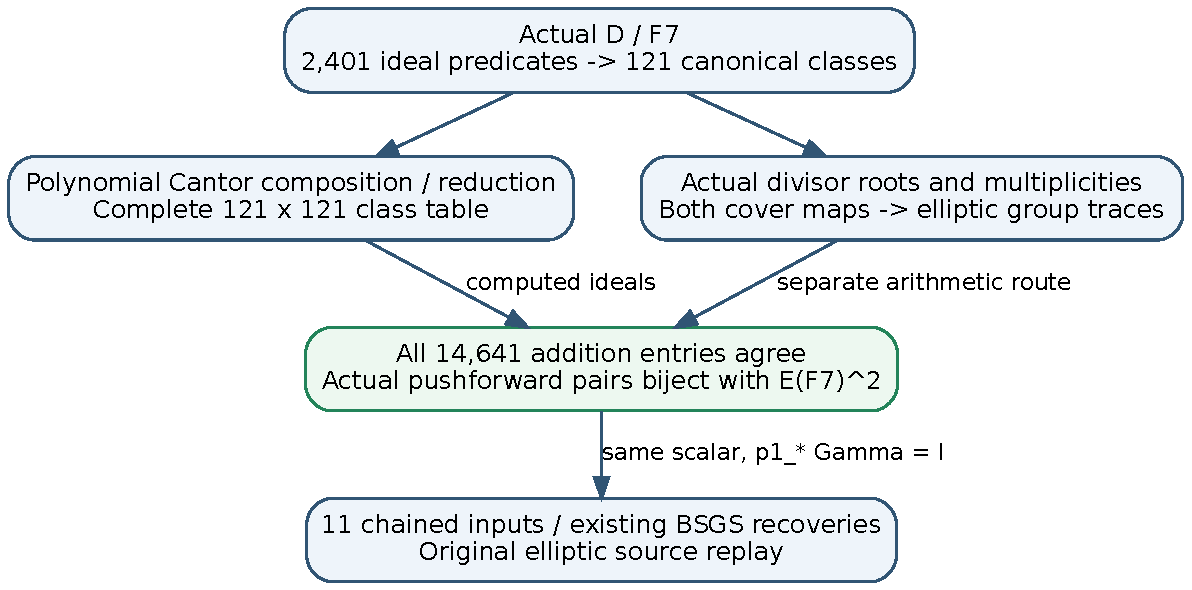
\includegraphics[width=\linewidth,height=81mm,keepaspectratio]{arithmetic.pdf}
\end{center}

\textbf{The infinity model fixes the representation.} The leading six is
nonsquare in $\mathbb F_7$; infinity consists of two conjugate points,
$\eta^2=6$. Their rational sum $D_\infty$ is canonical: $dW/Y$ has one
zero on each branch and none on the affine chart. Riemann--Roch gives
every nonzero rational class a unique affine semi-reduced degree-two
representative relative to $D_\infty$. An infinity component would force
both branches and the zero class; a full hyperelliptic fibre is also
canonical. Thus each nonzero class has a monic quadratic $u$, linear
$v$, and $u\mid H-v^2$. The identity alone is $(1,0)$.
This uses the actual divisor base, rather than a single rational infinity
or product-group labels. [pcc:unverified]

\textbf{A complete fixed population.} All $49\cdot49=2401$ candidate
ideals are tested. Accepted classes comprise 84 split packets, 14 repeated
rational-point packets, 22 irreducible quadratic packets and the identity.
Their two actual cover pushforwards give every ordered pair in
$E(\mathbb F_7)^2$ once. This agrees with the actual degree-four E-square
isogeny and rational group $C_{11}^2$. A matching population count alone
would not establish the divisor operation. [pcc:unverified]

\newpage
{\Large\bfseries Genuine class operations, scalar interface and original evidence}\par

\textbf{Balanced Cantor law.} Each composition retains an exact monic
three-term Bezout identity for
\[
d=\gcd(u_1,u_2,v_1+v_2),\qquad u=u_1u_2/d^2,
\]
with exact divisions for $u$ and its interpolating $v$. The composed
degree is zero, two or four. At degree four,
\[
u'=\operatorname{monic}((H-v^2)/u),\quad v'=-v\bmod u',\qquad
6-v_3^2\in\{6,5,2,4\}\ne0.
\]
Both infinity pole orders of $Y-v$ are three, so its full principal
divisor gives the required sum relative to $D_\infty$. Equal infinity
counterweights eliminate an extra balancing step. The actual quotient
and curve congruence are checked at every addition. The complete table
also passes identity, inverse, commutativity, exponent eleven and all
1,771,561 associativity triples. [pcc:unverified]

\textbf{The comparison route evaluates the covers.} Split/repeated roots
are evaluated with their true multiplicities. An irreducible quadratic
uses its own quotient field, all norm inverses and Frobenius identities;
its two cover images are added on $E$ and descend to the base field.
At $W=0$, $p_2=O$ through its proper extension. At infinity,
$p_{1*}D_\infty=2O$ and $p_{2*}D_\infty=(0,\eta)+(0,-\eta)=O$.
No base correction, exceptional root or repeated point is omitted.
The Cantor code never uses the resulting pair as its answer.
[pcc:unverified]

\textbf{All eleven transfer and recovery cases.} With $A=p_1^*$ and
$B=p_2^*$, compute $\Gamma(P)=[6](A(P)+B([-2]P))$ from input points.
Every case has pushforwards $(P,[-2]P)$ and commutes with scalar
multiplication from $T$. The existing Shanks baby-step giant-step
function receives only a Mumford base, target and order eleven. The
known oracle remains in the driver; returned scalars replay on the
original elliptic curve. The integral global map/retraction comes from
crypto 5114's quotient argument, not from inverse two modulo eleven.
This is a toy interface check without authenticated blindness or timing.
[pcc:unverified]

\begin{center}\small
\begin{tabular}{ll}
\toprule
Frozen source / protocol / lock & f9b1f332 / d648db / 674f2c\\
Complete pre-call published input readback & 43 inputs plus lock, 44 whole files\\
Strict phases / post-call guards & 7 of 7 pass / unchanged\\
Whole native stdout / classes / Cayley table & 3390 / 4875 / 46010 bytes\\
Whole small original records retained & 40\\
Original ELF and separate 0555 qualifier & 4733416 bytes each; hash prefix f28eeac9\\
\bottomrule
\end{tabular}\end{center}
Pinned Rust 1.99.1, warnings as errors, opt3, overflow/debug assertions,
120 seconds/2 GiB/one worker per phase. Every source/copy/tool/named
runtime/qualifier guard agrees. Whole original large binaries remain
RAM pending approved custody; new CI originals are distinct.
[pcc:unverified]

\textbf{Real controls.} Changing $H_0$ or an actual pullback $u_0$ fails
the curve congruence. Negating an actual sum's $v$ gives a valid inverse,
correctly rejected as the original addition answer. Changing the actual
chain scalar six to five breaks its left-inverse identity. All pristine
relations restore. There is no strict/native mathematical or resource
failure in first A. Earlier bootstrap, sparse-index, line-count and
source-access metadata negatives remain preserved. [pcc:unverified]

\textbf{Prior work and scope.} The read primary balanced-arithmetic paper
is Galbraith--Harrison--Mireles Morales (ANTS 2008), sections 2--4,
especially the even-genus nonsplit case on page 352. Galbraith's corrected
chapter 10 supplies the full affine composition/reduction arguments.
The original Cantor AMS PDF returned 403 and was not treated as read.
Generic crypto-lean 38 retains two pre-check private-import failures,
zero accepted theorems and no axiom-audit pass. Full faithful Lean actual
geometry/algorithm and signed independent verification remain open.
The original unpriced solver assessment is unchanged; no benchmark,
registry or IC leaderboard transition occurs. Next is the genuine
degree-three dual cover, where Frobenius acts by seventh powers on
function fields. [pcc:unverified]
\end{document}
